\section{Application and Reproducibility}
\subsection{Relative depth-based background blur}
The application turns relative ordering into an artistic blur effect. Using DA's fixed whole-clip display limits $(L,H)$, let
\begin{align}
u&=\operatorname{clip}((r-L)/(H-L),0,1),\\
v&=\operatorname{clip}((u-0.45)/(0.70-0.45),0,1),\\
\beta&=1-(3v^2-2v^3).
\end{align}
We blend $\beta\,\mathcal G_5(I)+(1-\beta)I$, where $\mathcal G_5$ is Gaussian blur with 5-pixel standard deviation. Larger relative inverse depth retains sharp near content; smaller values blur farther content. Invalid predictions leave RGB unchanged. Raw DA and E4 use identical limits and effect parameters.

\begin{figure*}[t]
\centering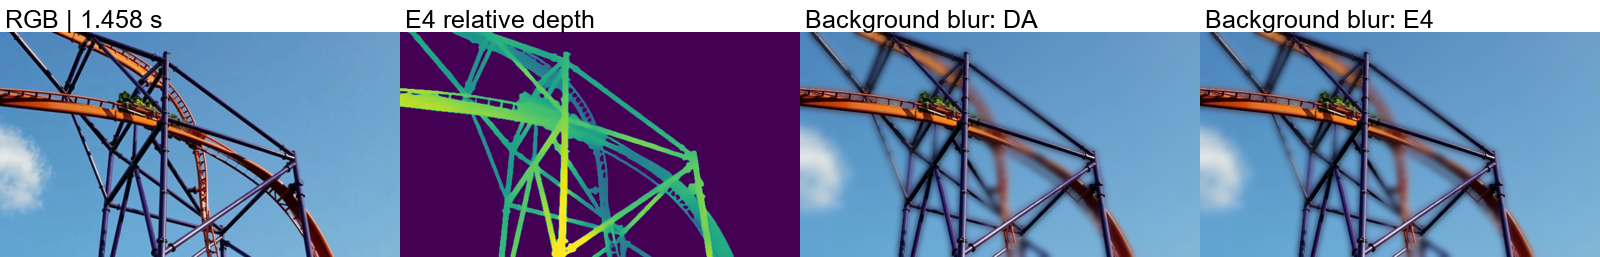
\includegraphics[width=\textwidth]{images/application.png}
\caption{Recorded application at test frame 35: RGB, E4 relative depth, raw-DA blur, and E4 blur. Shared effect settings isolate the changed depth input. The effect is not a calibrated aperture simulation; edge halos and incorrect foreground/background decisions remain possible.}
\label{fig:application}
\end{figure*}
The recorded demonstration contains every original test timestamp and all 70 frames. Figure~\ref{fig:application} shows stronger retention of near supports and blur on farther content. DA and E4 effects are visually close, so we do not claim a large perceptual improvement in this application. A blur applied before compositing can bleed color across a boundary; a wrong depth ordering can blur the wrong object. Proper layered compositing and explicit user focus selection would be extensions rather than evidence already delivered.

\subsection{Verification and handover}
All stages retain source hashes and floating-point outputs. Verification recomputes every saved flow field, common mask, E0--E4 prediction and history weight, and E0--E5 score. NYUv2 requires the standard 654 IDs and unchanged RGB/GT/prediction hashes. Stereo auditing reproduces the positive-disparity GT regions, MAE, and valid fractions for all 15 pairs.

Exports are decoded again to check every timestamp and frame count. The blur effect is recomputed from saved arrays before encoding. Analytical tests cover crop/clipping, strict thresholds, known motion, warp direction, invalid interpolation, relative affine invariance, and near/far blur response. These establish implementation contracts rather than experimental accuracy.

The ZIP contains development and frozen test comparisons, ablations, application footage, timestamps, source metadata, selection evidence, and case indices. Every payload is checked by SHA256 after writing, in addition to ZIP CRC. Code and compact results are versioned on GitHub; large inputs and raw predictions remain local. Personal acceptance notes, weights, and datasets are excluded from the archive. The report and ZIP are separate deliverables; no course submission or optional arXiv publication has been performed.

Nominal module ownership remains Qinchuan XIAO for data, geometry, metric evaluation, and fusion, and Jun Yu Eugene YIP for video models, temporal/efficiency experiments, and the application. The implementation and experiments were assisted by an AI coding agent. Automated verification and assistant visual review do not imply either member has independently reproduced or accepted the result.
